%%%%%%%%%%%%%%%%%%%%%%%%%%%%%%%%%%%%%%%%%%%%%%%%%%%%%%%%%%%%%%%%%%%%%%
%     File: ExtendedAbstract_resul.tex                               %
%     Tex Master: ExtendedAbstract.tex                               %
%%%%%%%%%%%%%%%%%%%%%%%%%%%%%%%%%%%%%%%%%%%%%%%%%%%%%%%%%%%%%%%%%%%%%%

\section{Experiments}
\label{sec:experiments}

This section presents a comprehensive experimental evaluation of Aerial-D that spans model training, cross-dataset generalization, and targeted ablations. We first describe the model architecture and training setup, then report cross-dataset results on established aerial referring segmentation benchmarks. Beyond aggregate performance, we also include: (i) ablation of expression enhancement strategies; (ii) ablation of historic-filter training; and (iii) qualitative comparison across language models (o3, base Gemma3, and our distilled Gemma3-Aerial model), coupled with a cost analysis of these alternatives.

\subsection{Model Architecture}
\label{subsec:model_architecture}

In selecting the architecture for our experiments, we prioritized a model that can interpret natural-language descriptions while producing pixel-accurate masks in aerial scenes. Generic segmentation systems rarely meet both requirements under the domain shift of remote sensing, where objects are small, repetitive, and densely arranged. We therefore adopt RSRefSeg as our backbone for referring segmentation: it pairs a strong language–image encoder (SigLIP2) with a state-of-the-art mask decoder (SAM), enabling robust semantic grounding alongside precise mask generation, and we adapt it to the remote-sensing domain using LoRA for parameter-efficient fine-tuning. This choice is further supported by the strong performance reported for RSRefSeg on RRSIS-D\cite{liu2024rotated}, providing a proven baseline for aerial referring segmentation and reducing risk in our evaluation.

Concretely, we implement the RSRefSeg architecture\cite{chen2025rsrefseg} in PyTorch, as illustrated in Figure~\ref{fig:rsrefseg_arch}. The design couples SigLIP2\cite{siglip2} for vision–language encoding with SAM\cite{sam} for mask generation. We adopt LoRA (Low-Rank Adaptation)\cite{lora} for parameter‑efficient fine‑tuning while preserving the strong pretraining of both backbones. In practice, we adapt the query and value projection layers in the vision encoders and the query, key, value, and output projection layers in the text encoder.

\subsection{Experimental Setup}
\label{subsec:experimental_setup}

Our training configuration uses a batch size of 4 with gradient accumulation steps of 2, achieving an effective batch size of 8 samples. The model employs \texttt{SigLIP2-SO400M} for vision–language encoding and \texttt{SAM-ViT-Large} for mask generation when training the combined model. We adopt LoRA with rank \(r=32\) for parameter-efficient adaptation. Training uses AdamW optimizer\cite{adamw} with initial learning rate of 1e-4, weight decay of 0.01, and polynomial learning rate decay with power factor 0.9. Mixed-precision computation and gradient clipping with maximum norm of 1.0 ensure training stability. All images are resized to 384×384 pixels to match SigLIP2 input requirements. Historic filters are applied to 20\% of training images; for each selected image, one of three variants—grayscale, grain/contrast roll-off, or sepia/noise—is chosen uniformly at random (probability 1/3 each).

We train a single combined model on all five datasets—Aerial-D, RRSIS-D\cite{liu2024rotated}, NWPU-Refer\cite{yang2024large}, RefSegRS\cite{yuan2023rrsis}, and Urban1960SatSeg\cite{hao2025urban1960satseg}—and evaluate on these same five datasets. To assess robustness under degradation beyond our own data, we also report results on historic-filtered variants of the three non-historic external datasets (RRSIS-D, NWPU-Refer, RefSegRS). In addition, to study generalization to a lighter decoder, we evaluate a configuration using \texttt{SAM-ViT-Base} at test time.

\subsection{Evaluation Results}
\label{subsec:evaluation_results}

Our evaluation demonstrates the effectiveness of training a unified model on multiple datasets. The combined training performance evaluation in Table \ref{tab:combined_training_results} shows our main experimental results, where the model is trained on all five datasets (Aerial-D, RRSIS-D\cite{liu2024rotated}, NWPU-Refer\cite{yang2024large}, RefSegRS\cite{yuan2023rrsis}, and Urban1960SatSeg\cite{hao2025urban1960satseg}) and evaluated across different domains. This approach enables the model to leverage the diversity of expression styles and object categories across datasets while maintaining strong performance on each evaluation set.

% Combined training performance table
\begin{table*}[t]
\centering
\caption{Combined Training Performance Evaluation - Model Trained on All Dataset Train Sets (Historic-filtered results in \textcolor{blue}{blue})}
\label{tab:combined_training_results}
\begin{tabular}{@{}lcccccccc@{}}
\toprule
\textbf{Dataset} & \textbf{IoU@0.5} & \textbf{IoU@0.7} & \textbf{IoU@0.9} & \multicolumn{2}{c}{\textbf{mIoU}} & \multicolumn{2}{c}{\textbf{oIoU}} \\
\cmidrule(lr){5-6} \cmidrule(lr){7-8}
 & & & & \textbf{Orig.} & \textbf{Hist.} & \textbf{Orig.} & \textbf{Hist.} \\
\midrule
Aerial-D & -- & -- & -- & -- & \textcolor{blue}{--} & -- & \textcolor{blue}{--} \\
RRSIS-D & 68.51\% & 53.16\% & 18.74\% & 60.01\% & \textcolor{blue}{55.20\%} & 71.48\% & \textcolor{blue}{68.26\%} \\
NWPU-Refer & 38.64\% & 25.68\% & 6.64\% & 35.81\% & \textcolor{blue}{30.17\%} & 51.77\% & \textcolor{blue}{48.31\%} \\
RefSegRS & 36.43\% & 9.74\% & 1.39\% & 36.75\% & \textcolor{blue}{24.53\%} & 44.41\% & \textcolor{blue}{30.21\%} \\
Urban1960SatSeg & 74.80\% & 58.74\% & 28.46\% & 67.72\% & N/A & 86.43\% & N/A \\
\bottomrule
\end{tabular}
\end{table*}


\subsection{Expression Enhancement Ablation}
\label{subsec:ablation_studies}

To evaluate the individual contributions of different expression enhancement strategies, we conduct an ablation study comparing models trained on different subsets of Aerial-D. The primary motivation is to determine whether the LLM enhancement process positively impacts model performance and to quantify the benefits of each enhancement type. Our training set contains approximately 371K rule-based expressions, 364K language variation expressions, and 382K unique visual detail expressions, totaling 1.12M training expressions.

To ensure fair comparison across training configurations, we carefully control the total number of training samples each model observes. The individual subset models train for multiple epochs to match the sample count of the combined dataset trained for fewer epochs, preventing performance differences from arising simply from training data quantity rather than quality and diversity.

% Ablation expression types table with explicit epochs and samples
\begin{table*}[t]
\centering
\caption{Expression Enhancement Ablation Across Four Datasets}
\label{tab:ablation_expression_types}
\resizebox{\textwidth}{!}{%
\begin{tabular}{@{}lcc|cc|cc|cc|cc@{}}
\toprule
\multirow{2}{*}{\textbf{Training Configuration}} & \multirow{2}{*}{\textbf{Samples}} & \multirow{2}{*}{\textbf{Epochs}} & \multicolumn{2}{c|}{\textbf{Aerial-D}} & \multicolumn{2}{c|}{\textbf{RefSegRS}} & \multicolumn{2}{c|}{\textbf{RRSIS-D}} & \multicolumn{2}{c}{\textbf{NWPU-Refer}} \\
\cmidrule(lr){4-5} \cmidrule(lr){6-7} \cmidrule(lr){8-9} \cmidrule(lr){10-11}
 & & & % \textbf{Pass@0.7} & 
\textbf{mIoU} & \textbf{oIoU} & % \textbf{Pass@0.7} & 
\textbf{mIoU} & \textbf{oIoU} & % \textbf{Pass@0.7} & 
\textbf{mIoU} & \textbf{oIoU} & % \textbf{Pass@0.7} & 
\textbf{mIoU} & \textbf{oIoU} \\
\midrule
Rule-based Only & 371K & 4 & % 26.81\% & 
34.57\% & 39.31\% & % 2.55\% & 
3.73\% & 0.55\% & % 29.89\% & 
34.22\% & 36.46\% & % 13.62\% & 
16.78\% & 13.70\% \\
Enhanced Only & 364K & 4 & % 36.39\% & 
46.45\% & 56.99\% & % \textbf{3.02\%} & 
5.75\% & 4.99\% & % \textbf{35.63\%} & 
\textbf{41.63\%} & \textbf{42.48\%} & % \textbf{16.90\%} & 
21.89\% & 16.68\% \\
Unique Expressions Only & 382K & 4 & % 35.75\% & 
46.54\% & 63.02\% & % 2.55\% & 
18.32\% & 8.37\% & % 20.86\% & 
31.78\% & 33.73\% & % 15.91\% & 
\textbf{24.68\%} & \textbf{29.22\%} \\
Combined All & 1,118K & 2 & % \textbf{39.54\%} & 
\textbf{49.33\%} & \textbf{64.30\%} & % 1.86\% & 
\textbf{18.80\%} & \textbf{8.58\%} & % 23.39\% & 
34.07\% & 34.80\% & % 15.91\% & 
24.57\% & 28.27\% \\
\bottomrule
\end{tabular}%
}
\end{table*}

The results demonstrate that the combined model, utilizing all expression types, achieves the best performance across evaluation metrics on Aerial-D. Notably, different subsets show varying benefits for different target datasets: Enhanced Only performs best on RRSIS-D, while Unique Expressions Only excels on NWPU-Refer. This indicates that smaller, focused subsets can be more data-efficient and faster to train than the full combined dataset, while still achieving competitive or superior performance on specific target domains.


\subsection{Distillation Ablation: Gemma3 vs. o3 Model Comparison}
\label{subsec:distillation_ablation}

In order to obtain high-quality language supervision without incurring prohibitive annotation costs, we distill from o3 into a local Gemma3 model and evaluate the impact of removing that distillation. The challenge is that proprietary models like o3 yield strong expressions but are expensive at scale, while an unadapted Gemma3 base model can hallucinate or miss domain-specific cues in aerial imagery. We therefore compare three sources of expressions: direct o3 outputs, the vanilla Gemma3 base, and our Gemma3-Aerial model distilled from o3 using 500 samples.

This ablation shows that removing distillation degrades the accuracy and grounding of generated expressions: the vanilla Gemma3 model frequently references objects not present in the scene, whereas the distilled Gemma3-Aerial model consistently produces grounded descriptions that align with visible structures and simple spatial relations. At the same time, distillation dramatically reduces cost while preserving the qualitative benefits of stronger supervision.

Figure \ref{fig:distillation_comparison} presents representative examples of this comparison across various aerial scenes and object categories. The results clearly illustrate how the fine-tuned model learned to avoid common hallucination patterns while maintaining the linguistic diversity and natural language quality that make the expressions useful for training robust segmentation models.

% Cost comparison table
\begin{table}[t]
\centering
\caption{Cost Analysis: Gemma3 vs. o3 Model for Large-Scale Annotation\protect\footnotemark}
\label{tab:cost_comparison}
\resizebox{\columnwidth}{!}{%
\begin{tabular}{@{}lcc@{}}
\toprule
\textbf{Model} & \textbf{Cost per request} & \textbf{Cost for 300K requests} \\
\midrule
o3 Model & \$0.020728 & \$6,218.32 \\
Distilled Gemma3 & \$0.000087 & \$26.01 \\
\midrule
\textbf{Savings} & \textbf{238× cheaper} & \textbf{\$6,192.31 (99.6\%)} \\
\bottomrule
\end{tabular}%
}
\end{table}
\footnotetext{Cost calculations based on API pricing — o3: \$2.00 per million input tokens, \$8.00 per million output tokens (OpenAI API platform); Gemma3-12B: \$0.035 per million input tokens, \$0.141 per million output tokens (OpenRouter inference provider). Average tokens per request: o3 (1,670.8 input, 2,173.3 output), Gemma3 (1,330.0 input, 284.7 output). Calculations based on 15 sample requests.}

The cost analysis demonstrates that using the distilled Gemma3 model provides substantial economic advantages for large-scale dataset generation. The upfront investment in distillation training pays off significantly when generating millions of annotations, making the approach both technically sound and economically viable for scaling to larger datasets.

\begin{figure*}[t]
\centering
\begin{minipage}{0.5\textwidth}
\centering
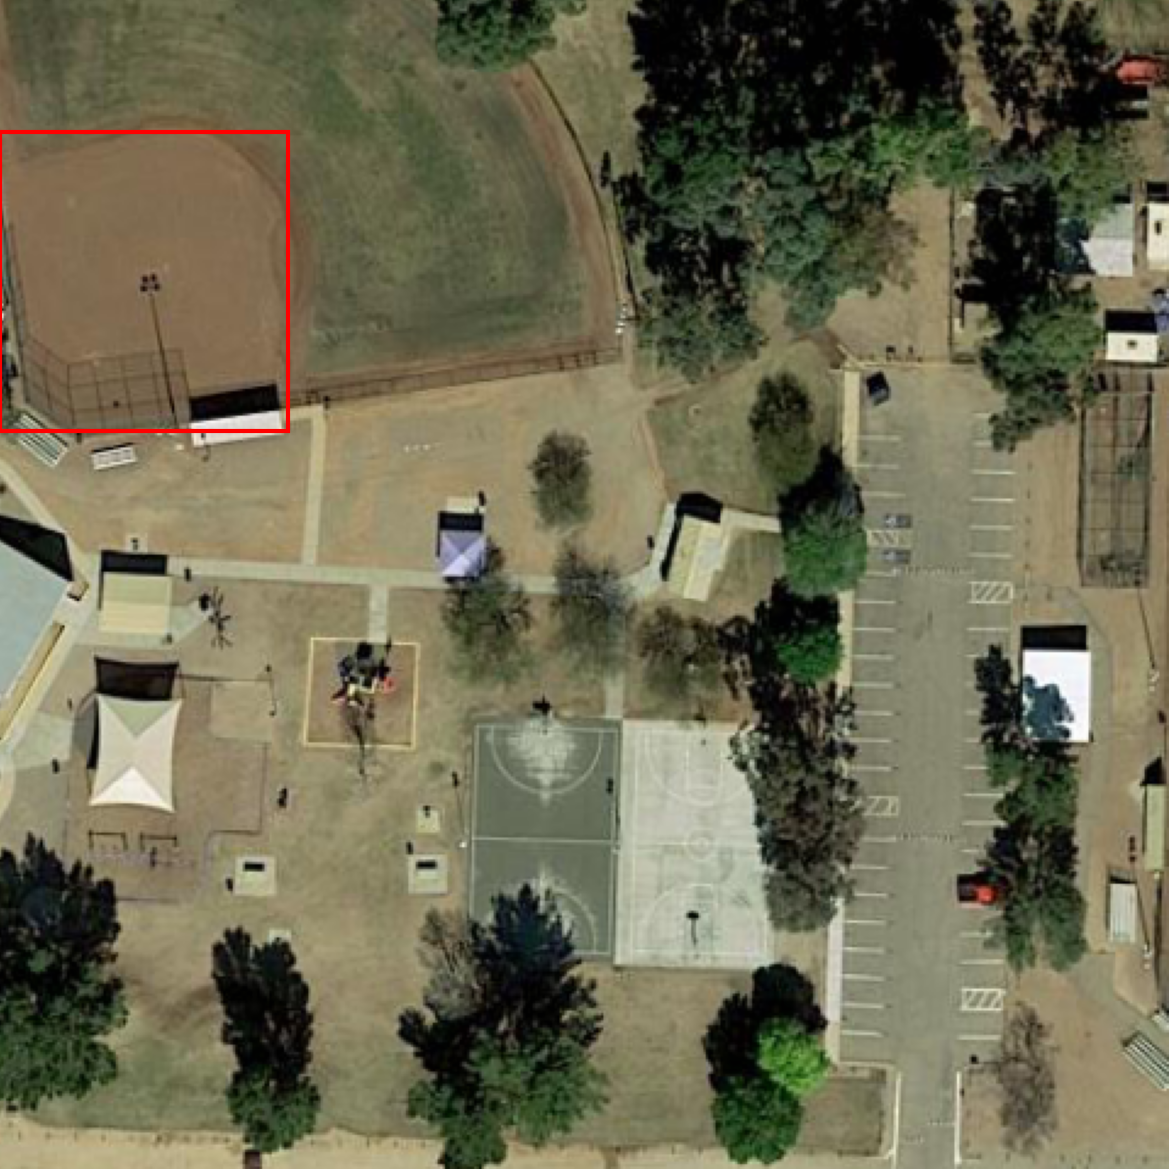
\includegraphics[width=0.65\textwidth]{./images/3llm.png}
\end{minipage}%
\begin{minipage}{0.5\textwidth}
\centering
\hspace{-1cm}
\raisebox{-0.3\height}{%
\footnotesize
\begin{tabular}{@{}p{2cm}p{5cm}@{}}
\toprule
\textbf{Expression Type} & \textbf{Example} \\
\midrule
Original & the orange baseball diamond in the top left \\
\midrule
o3 Enhanced & the orange baseball diamond with the light pole near home plate in the upper left \\
\midrule
Gemma3 Base & the bright orange baseball diamond to the left of another similar baseball diamond in the top left \\
\midrule
Gemma3-Aerial-12B & the orange baseball field with a chainlink fence surrounded by grass to the north and trees to the west \\
\bottomrule
\end{tabular}%
}
\end{minipage}
\caption{Qualitative comparison between o3, vanilla Gemma3 base model, and our fine-tuned Gemma3-Aerial-12B model on aerial imagery. The table shows how each model enhances the original rule-based expression, demonstrating the progression from basic rule-based descriptions through various levels of language model enhancement.}
\label{fig:distillation_comparison}
\end{figure*}


\subsection{Historic Filter Ablation Study}
\label{subsec:historic_ablation}

To better handle degraded conditions typical of historical aerial imagery, we ablate the use of historic filters during training. Models trained exclusively on modern imagery often fail under reduced contrast, film grain, or monochrome tones; therefore, we compare training with and without on-the-fly filter augmentation while holding other factors constant. We train on Aerial-D, RRSIS-D, NWPU-Refer, RefSegRS, and Urban1960SatSeg, but suppress filters on the first four datasets (only Urban1960SatSeg inherently contains historic imagery). The results in Table \ref{tab:historic_ablation_results} show that historic-filter augmentation improves robustness on degraded test conditions without compromising performance on original imagery.

% Historic filter ablation table
\begin{table*}[t]
\centering
\caption{Historic Filter Ablation Study - Model Trained on All Datasets Without Historic Filters (except UrbanSatSeg1960)}
\label{tab:historic_ablation_results}
\begin{tabular}{@{}lcccccccc@{}}
\toprule
\textbf{Dataset} & \textbf{IoU@0.5} & \textbf{IoU@0.7} & \textbf{IoU@0.9} & \multicolumn{2}{c}{\textbf{mIoU}} & \multicolumn{2}{c}{\textbf{oIoU}} \\
\cmidrule(lr){5-6} \cmidrule(lr){7-8}
 & & & & \textbf{Orig.} & \textbf{Hist.} & \textbf{Orig.} & \textbf{Hist.} \\
\midrule
Aerial-D & -- & -- & -- & -- & \textcolor{blue}{--} & -- & \textcolor{blue}{--} \\
RRSIS-D & -- & -- & -- & -- & \textcolor{blue}{--} & -- & \textcolor{blue}{--} \\
NWPU-Refer & -- & -- & -- & -- & \textcolor{blue}{--} & -- & \textcolor{blue}{--} \\
RefSegRS & -- & -- & -- & -- & \textcolor{blue}{--} & -- & \textcolor{blue}{--} \\
Urban1960SatSeg & -- & -- & -- & -- & N/A & -- & N/A \\
\bottomrule
\end{tabular}
\end{table*}
